\chapter{Análisis y Trazado de las Rectas de Carga}
\label{chap:rectas_de_carga}

En este capítulo se realiza el cálculo y trazado de las rectas de carga. Este método permite visualizar y determinar
los límites físicos de excursión de señal, previniendo la distorsión por recorte en la zona de corte o en la zona
de triodo del transistor.

\section{Recta de Carga Estática de Corriente Continua}

La recta de carga de continua (CC) describe la relación lineal entre la corriente de drenador ($i_D$) y la tensión
drenador-surtidor ($v_{DS}$) impuesta por la malla exterior del circuito en ausencia de excitación dinámica, donde los
capacitores $C_1, C_2$ y $C_3$ actúan como circuitos abiertos.

La ecuación de malla de salida en continua viene dada por:
\begin{equation}
  V_{DD} = v_{DS} + i_D \cdot (R_D + R_S) = v_{DS} + i_D \cdot R_{CC}
  \label{eq:malla_salida_cc}
\end{equation}
donde la resistencia estática total de continua es:
\begin{equation}
  R_{CC} = R_D + R_S = 6.8\kohm + 1.5\kohm = 8.3\kohm = 8300\ohm
  \label{eq:Rcc_tp5}
\end{equation}

Despejando la corriente de drenador en función de la tensión:
\begin{equation}
  i_D = -\frac{1}{R_{CC}} \cdot v_{DS} + \frac{V_{DD}}{R_{CC}} = -\frac{1}{8.3\kohm} \cdot v_{DS} + \frac{15.0\V}{8.3\kohm}
  \label{eq:recta_cc_tp5}
\end{equation}

Los puntos de intersección con los ejes coordenados resultan:
\begin{enumerate}
  \item Intersección con el eje de abscisas ($i_D = 0$, tensión de corte estático):
    \begin{equation}
      V_{DS,\mathrm{corte(CC)}} = V_{DD} = 15.00\V \implies (15.0\V,\, 0\mA)
    \end{equation}
  \item Intersección con el eje de ordenadas ($v_{DS} = 0$, corriente de saturación estática):
    \begin{equation}
      I_{D,\mathrm{sat(CC)}} = \frac{V_{DD}}{R_{CC}} = \frac{15.0\V}{8300\ohm} \approx 1.807\mA \implies (0\V,\, 1.807\mA)
    \end{equation}
\end{enumerate}

La pendiente de la recta estática es $m_{CC} = -1/R_{CC} = -1.205 \times 10^{-4}\,\Omega^{-1}$.

\section{Recta de Carga Dinámica de Corriente Alterna}

A la frecuencia de excitación ($1\kHz$), los capacitores electrolíticos de acoplo y desacoplo ($100\uF$) exhiben una
reactancia capacitiva despreciable:
\begin{equation}
  X_C = \frac{1}{2\pi \cdot f \cdot C} = \frac{1}{2\pi \cdot 1000\Hz \cdot 100\uF} \approx 1.59\ohm \ll R_S, R_L
\end{equation}
comportándose efectivamente como cortocircuitos ideales para la señal de alterna.

Por lo tanto, el terminal de surtidor queda conectado dinámicamente a la masa de alterna a través de $C_2$, anulando
el efecto resistivo de $R_S$. Simultáneamente, el capacitor $C_3$ conecta la resistencia de carga $R_L = 10\kohm$ en
paralelo con el resistor de drenador $R_D = 6.8\kohm$. La resistencia dinámica equivalente de carga resulta:
\begin{equation}
  R_{CA} = R_D \parallel R_L = \frac{6.8\kohm \cdot 10\kohm}{6.8\kohm + 10\kohm} = \frac{68}{16.8}\kohm \approx 4.0476\kohm \approx 4.048\kohm
  \label{eq:Rca_tp5}
\end{equation}

La recta dinámica de alterna pasa obligatoriamente por el punto de reposo $Q(V_{DSQ} = 6.927\V, I_{DQ} = 0.9727\mA)$
y su pendiente viene determinada por $-1/R_{CA}$. La ecuación punto-pendiente se formula como:
\begin{equation}
  i_D - I_{DQ} = -\frac{1}{R_{CA}} \cdot (v_{DS} - V_{DSQ})
\end{equation}
reescribiéndose en forma explícita:
\begin{equation}
  i_D = -\frac{1}{R_{CA}} \cdot v_{DS} + \left(I_{DQ} + \frac{V_{DSQ}}{R_{CA}}\right)
  \label{eq:recta_ca_tp5}
\end{equation}

Los puntos singulares de la recta dinámica son:
\begin{enumerate}
  \item Tensión de corte dinámica ($i_D = 0$):
    \begin{equation}
      \begin{aligned}
        V_{DS,\max(\mathrm{CA})} &= V_{DSQ} + I_{DQ} \cdot R_{CA} \\
        &= 6.927\V + (0.9727\mA \cdot 4.0476\kohm) \approx 10.864\V
      \end{aligned}
    \end{equation}
    correspondiente al punto $(10.864\V,\, 0\mA)$.
  \item Corriente de saturación dinámica ($v_{DS} = 0$):
    \begin{equation}
      \begin{aligned}
        I_{D,\max(\mathrm{CA})} &= I_{DQ} + \frac{V_{DSQ}}{R_{CA}} \\
        &= 0.9727\mA + \frac{6.927\V}{4.0476\kohm} \approx 2.6841\mA
      \end{aligned}
    \end{equation}
    correspondiente al punto $(0\V,\, 2.684\mA)$.
\end{enumerate}

La pendiente dinámica es $m_{CA} = -1/R_{CA} \approx -2.471 \times 10^{-4}\,\Omega^{-1}$, notablemente más pronunciada
que la pendiente estática debido al acoplamiento de la carga en paralelo.

\section{Frontera de Triodo y Excursión Dinámica Máxima}

Para garantizar la amplificación lineal, el canal del MOSFET debe permanecer estrangulado en todo el ciclo de la señal,
evitando ingresar a la región de triodo (óhmica). El límite físico está fijado por la condición:
\begin{equation}
  v_{DS} \ge v_{GS} - V_{th}
\end{equation}
En el punto de trabajo estático, el exceso de compuerta es:
\begin{equation}
  V_{DS,\mathrm{sat}} = V_{GSQ} - V_{th} = 1.791\V - 1.601\V = 0.190\V
\end{equation}

Evaluando los márgenes de oscilación posibles alrededor del punto de reposo $Q$:
\begin{itemize}
  \item Margen hacia la zona de corte:
    \begin{equation}
      \Delta v_{o,\mathrm{corte}} = I_{DQ} \cdot R_{CA} = 0.9727\mA \cdot 4.0476\kohm \approx 3.937\V_p \implies 7.874\Vpp
    \end{equation}
  \item Margen hacia la zona de triodo:
    \begin{equation}
      \Delta v_{o,\mathrm{triodo}} = V_{DSQ} - V_{DS,\mathrm{sat}} = 6.927\V - 0.190\V = 6.737\V_p \implies 13.474\Vpp
    \end{equation}
\end{itemize}

El límite estricto de excursión simétrica viene impuesto por la aproximación al corte dinámico, fijando una amplitud pico
máxima admisible de salida de:
\begin{equation}
  \hat{v}_{o,\max} = 3.937\V_p \implies \hat{v}_{o,\max(\mathrm{pp})} \approx 7.87\Vpp
\end{equation}

Refiriendo este valor a los terminales de entrada a través de la ganancia de tensión ($|A_v| \approx 42.9$):
\begin{equation}
  \hat{v}_{i,\max} = \frac{\hat{v}_{o,\max}}{|A_v|} = \frac{3.937\V}{42.91} \approx 91.75\mV_p \implies 183.5\mVpp
\end{equation}

Dado que en las simulaciones se aplicó una entrada de $45\mV_p$ ($90\mVpp$) y en los ensayos de banco una señal de
$50\mV_p$ ($100\mVpp$), la excursión dinámica demandada representa apenas el $54\%$ del límite de recorte.

En la figura~\ref{fig:plot_rectas_de_carga} se ilustran conjuntamente las rectas de carga estática y dinámica, el punto
de reposo $Q$ y la frontera con la zona de triodo.

\begin{figure}[!ht]
  \centering
  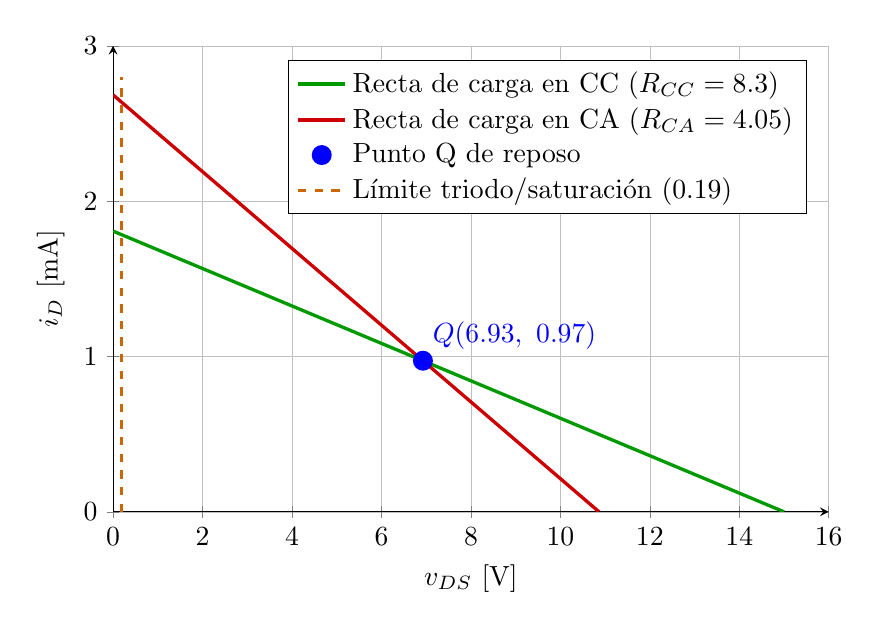
\begin{tikzpicture}
  \begin{axis}[
    width=0.88\textwidth,
    height=7.5cm,
    xlabel={$v_{DS}\ [\mathrm{V}]$},
    ylabel={$i_D\ [\mathrm{mA}]$},
    xmin=0, xmax=16.0,
    ymin=0, ymax=3.0,
    grid=both,
    grid style={line width=.1pt, draw=gray!30},
    major grid style={line width=.2pt, draw=gray!50},
    axis lines=left,
    legend pos=north east,
    legend cell align={left},
    every axis plot/.append style={very thick}
  ]
    % Recta de carga estatica (CC): i_D = (15 - x) / 8.3
    \addplot[domain=0:15.0, color=green!60!black, samples=2] {(15.0 - x) / 8.3};
    \addlegendentry{Recta de carga en CC ($R_{CC} = 8.3\kohm$)}

    % Recta de carga dinamica (CA): i_D = 0.9727 + (6.927 - x) / 4.048
    \addplot[domain=0:10.864, color=red!80!black, samples=2] {0.9727 + (6.927 - x) / 4.048};
    \addlegendentry{Recta de carga en CA ($R_{CA} = 4.05\kohm$)}

    % Punto Q de reposo
    \addplot[only marks, mark=*, mark size=3pt, color=blue] coordinates {(6.927, 0.9727)};
    \addlegendentry{Punto Q de reposo}

    % Limite de zona de saturacion (VDS = VGS - Vth = 0.190 V)
    \addplot[dashed, color=orange!80!black, samples=2] coordinates {(0.190, 0) (0.190, 2.8)};
    \addlegendentry{Límite triodo/saturación ($0.19\V$)}

    % Anotaciones
    \node[above right, text=blue] at (axis cs:6.93, 0.98) {$Q(6.93\V,\ 0.97\mA)$};
  \end{axis}
\end{tikzpicture}

  \caption{Trazado de las rectas de carga estática (CC) y dinámica (CA) con indicación del punto Q y frontera de triodo.}
  \label{fig:plot_rectas_de_carga}
\end{figure}
